% Created by tikzDevice version 0.12 on 2019-08-24 14:36:58
% !TEX encoding = UTF-8 Unicode
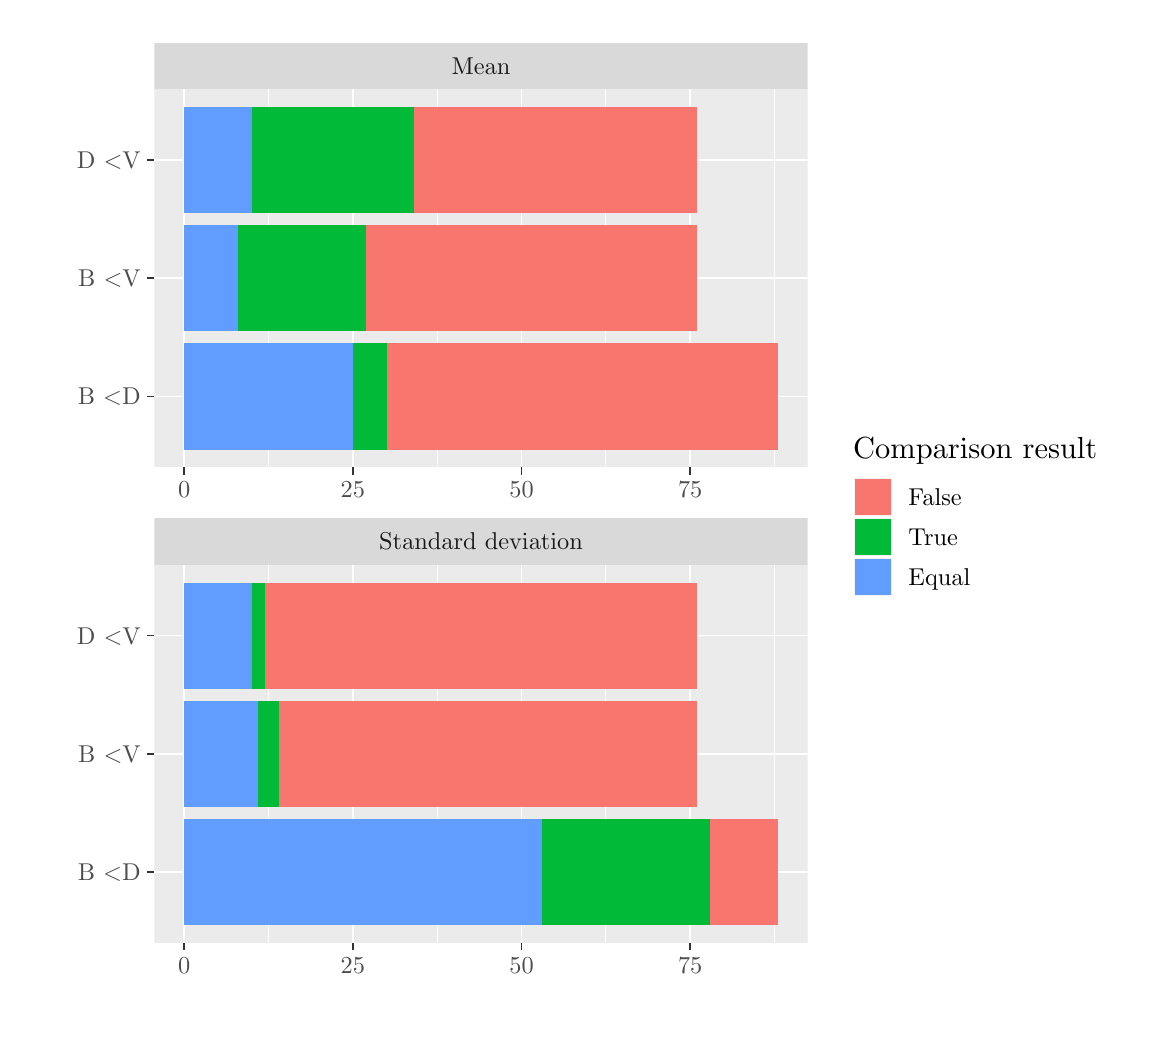
\begin{tikzpicture}[x=1pt,y=1pt]
\definecolor{fillColor}{RGB}{255,255,255}
\path[use as bounding box,fill=fillColor,fill opacity=0.00] (0,0) rectangle (397.48,361.35);
\begin{scope}
\path[clip] (  0.00,  0.00) rectangle (397.48,361.35);
\definecolor{drawColor}{RGB}{255,255,255}
\definecolor{fillColor}{RGB}{255,255,255}

\path[draw=drawColor,line width= 0.6pt,line join=round,line cap=round,fill=fillColor] (  0.00,  0.00) rectangle (397.48,361.35);
\end{scope}
\begin{scope}
\path[clip] ( 45.81,202.51) rectangle (281.82,339.05);
\definecolor{fillColor}{gray}{0.92}

\path[fill=fillColor] ( 45.81,202.51) rectangle (281.82,339.05);
\definecolor{drawColor}{RGB}{255,255,255}

\path[draw=drawColor,line width= 0.3pt,line join=round] ( 87.02,202.51) --
	( 87.02,339.05);

\path[draw=drawColor,line width= 0.3pt,line join=round] (147.97,202.51) --
	(147.97,339.05);

\path[draw=drawColor,line width= 0.3pt,line join=round] (208.92,202.51) --
	(208.92,339.05);

\path[draw=drawColor,line width= 0.3pt,line join=round] (269.88,202.51) --
	(269.88,339.05);

\path[draw=drawColor,line width= 0.6pt,line join=round] ( 45.81,228.11) --
	(281.82,228.11);

\path[draw=drawColor,line width= 0.6pt,line join=round] ( 45.81,270.78) --
	(281.82,270.78);

\path[draw=drawColor,line width= 0.6pt,line join=round] ( 45.81,313.45) --
	(281.82,313.45);

\path[draw=drawColor,line width= 0.6pt,line join=round] ( 56.54,202.51) --
	( 56.54,339.05);

\path[draw=drawColor,line width= 0.6pt,line join=round] (117.49,202.51) --
	(117.49,339.05);

\path[draw=drawColor,line width= 0.6pt,line join=round] (178.45,202.51) --
	(178.45,339.05);

\path[draw=drawColor,line width= 0.6pt,line join=round] (239.40,202.51) --
	(239.40,339.05);
\definecolor{fillColor}{RGB}{97,156,255}

\path[fill=fillColor] ( 56.54,208.91) rectangle (117.49,247.31);
\definecolor{fillColor}{RGB}{0,186,56}

\path[fill=fillColor] (117.49,208.91) rectangle (129.69,247.31);
\definecolor{fillColor}{RGB}{248,118,109}

\path[fill=fillColor] (129.69,208.91) rectangle (271.10,247.31);
\definecolor{fillColor}{RGB}{97,156,255}

\path[fill=fillColor] ( 56.54,251.58) rectangle ( 76.05,289.98);
\definecolor{fillColor}{RGB}{0,186,56}

\path[fill=fillColor] ( 76.05,251.58) rectangle (122.37,289.98);
\definecolor{fillColor}{RGB}{248,118,109}

\path[fill=fillColor] (122.37,251.58) rectangle (241.84,289.98);
\definecolor{fillColor}{RGB}{97,156,255}

\path[fill=fillColor] ( 56.54,294.25) rectangle ( 80.92,332.65);
\definecolor{fillColor}{RGB}{0,186,56}

\path[fill=fillColor] ( 80.92,294.25) rectangle (139.44,332.65);
\definecolor{fillColor}{RGB}{248,118,109}

\path[fill=fillColor] (139.44,294.25) rectangle (241.84,332.65);
\end{scope}
\begin{scope}
\path[clip] ( 45.81, 30.72) rectangle (281.82,167.26);
\definecolor{fillColor}{gray}{0.92}

\path[fill=fillColor] ( 45.81, 30.72) rectangle (281.82,167.26);
\definecolor{drawColor}{RGB}{255,255,255}

\path[draw=drawColor,line width= 0.3pt,line join=round] ( 87.02, 30.72) --
	( 87.02,167.26);

\path[draw=drawColor,line width= 0.3pt,line join=round] (147.97, 30.72) --
	(147.97,167.26);

\path[draw=drawColor,line width= 0.3pt,line join=round] (208.92, 30.72) --
	(208.92,167.26);

\path[draw=drawColor,line width= 0.3pt,line join=round] (269.88, 30.72) --
	(269.88,167.26);

\path[draw=drawColor,line width= 0.6pt,line join=round] ( 45.81, 56.32) --
	(281.82, 56.32);

\path[draw=drawColor,line width= 0.6pt,line join=round] ( 45.81, 98.99) --
	(281.82, 98.99);

\path[draw=drawColor,line width= 0.6pt,line join=round] ( 45.81,141.66) --
	(281.82,141.66);

\path[draw=drawColor,line width= 0.6pt,line join=round] ( 56.54, 30.72) --
	( 56.54,167.26);

\path[draw=drawColor,line width= 0.6pt,line join=round] (117.49, 30.72) --
	(117.49,167.26);

\path[draw=drawColor,line width= 0.6pt,line join=round] (178.45, 30.72) --
	(178.45,167.26);

\path[draw=drawColor,line width= 0.6pt,line join=round] (239.40, 30.72) --
	(239.40,167.26);
\definecolor{fillColor}{RGB}{97,156,255}

\path[fill=fillColor] ( 56.54, 37.12) rectangle (185.76, 75.52);
\definecolor{fillColor}{RGB}{0,186,56}

\path[fill=fillColor] (185.76, 37.12) rectangle (246.71, 75.52);
\definecolor{fillColor}{RGB}{248,118,109}

\path[fill=fillColor] (246.71, 37.12) rectangle (271.10, 75.52);
\definecolor{fillColor}{RGB}{97,156,255}

\path[fill=fillColor] ( 56.54, 79.79) rectangle ( 83.36,118.19);
\definecolor{fillColor}{RGB}{0,186,56}

\path[fill=fillColor] ( 83.36, 79.79) rectangle ( 90.68,118.19);
\definecolor{fillColor}{RGB}{248,118,109}

\path[fill=fillColor] ( 90.68, 79.79) rectangle (241.84,118.19);
\definecolor{fillColor}{RGB}{97,156,255}

\path[fill=fillColor] ( 56.54,122.46) rectangle ( 80.92,160.86);
\definecolor{fillColor}{RGB}{0,186,56}

\path[fill=fillColor] ( 80.92,122.46) rectangle ( 85.80,160.86);
\definecolor{fillColor}{RGB}{248,118,109}

\path[fill=fillColor] ( 85.80,122.46) rectangle (241.84,160.86);
\end{scope}
\begin{scope}
\path[clip] ( 45.81,167.26) rectangle (281.82,184.06);
\definecolor{fillColor}{gray}{0.85}

\path[fill=fillColor] ( 45.81,167.26) rectangle (281.82,184.06);
\definecolor{drawColor}{gray}{0.10}

\node[text=drawColor,anchor=base,inner sep=0pt, outer sep=0pt, scale=  0.88] at (163.82,172.63) {Standard deviation};
\end{scope}
\begin{scope}
\path[clip] ( 45.81,339.05) rectangle (281.82,355.85);
\definecolor{fillColor}{gray}{0.85}

\path[fill=fillColor] ( 45.81,339.05) rectangle (281.82,355.85);
\definecolor{drawColor}{gray}{0.10}

\node[text=drawColor,anchor=base,inner sep=0pt, outer sep=0pt, scale=  0.88] at (163.82,344.42) {Mean};
\end{scope}
\begin{scope}
\path[clip] (  0.00,  0.00) rectangle (397.48,361.35);
\definecolor{drawColor}{gray}{0.20}

\path[draw=drawColor,line width= 0.6pt,line join=round] ( 56.54, 27.97) --
	( 56.54, 30.72);

\path[draw=drawColor,line width= 0.6pt,line join=round] (117.49, 27.97) --
	(117.49, 30.72);

\path[draw=drawColor,line width= 0.6pt,line join=round] (178.45, 27.97) --
	(178.45, 30.72);

\path[draw=drawColor,line width= 0.6pt,line join=round] (239.40, 27.97) --
	(239.40, 30.72);
\end{scope}
\begin{scope}
\path[clip] (  0.00,  0.00) rectangle (397.48,361.35);
\definecolor{drawColor}{gray}{0.30}

\node[text=drawColor,anchor=base,inner sep=0pt, outer sep=0pt, scale=  0.88] at ( 56.54, 19.71) {0};

\node[text=drawColor,anchor=base,inner sep=0pt, outer sep=0pt, scale=  0.88] at (117.49, 19.71) {25};

\node[text=drawColor,anchor=base,inner sep=0pt, outer sep=0pt, scale=  0.88] at (178.45, 19.71) {50};

\node[text=drawColor,anchor=base,inner sep=0pt, outer sep=0pt, scale=  0.88] at (239.40, 19.71) {75};
\end{scope}
\begin{scope}
\path[clip] (  0.00,  0.00) rectangle (397.48,361.35);
\definecolor{drawColor}{gray}{0.20}

\path[draw=drawColor,line width= 0.6pt,line join=round] ( 56.54,199.76) --
	( 56.54,202.51);

\path[draw=drawColor,line width= 0.6pt,line join=round] (117.49,199.76) --
	(117.49,202.51);

\path[draw=drawColor,line width= 0.6pt,line join=round] (178.45,199.76) --
	(178.45,202.51);

\path[draw=drawColor,line width= 0.6pt,line join=round] (239.40,199.76) --
	(239.40,202.51);
\end{scope}
\begin{scope}
\path[clip] (  0.00,  0.00) rectangle (397.48,361.35);
\definecolor{drawColor}{gray}{0.30}

\node[text=drawColor,anchor=base,inner sep=0pt, outer sep=0pt, scale=  0.88] at ( 56.54,191.50) {0};

\node[text=drawColor,anchor=base,inner sep=0pt, outer sep=0pt, scale=  0.88] at (117.49,191.50) {25};

\node[text=drawColor,anchor=base,inner sep=0pt, outer sep=0pt, scale=  0.88] at (178.45,191.50) {50};

\node[text=drawColor,anchor=base,inner sep=0pt, outer sep=0pt, scale=  0.88] at (239.40,191.50) {75};
\end{scope}
\begin{scope}
\path[clip] (  0.00,  0.00) rectangle (397.48,361.35);
\definecolor{drawColor}{gray}{0.30}

\node[text=drawColor,anchor=base east,inner sep=0pt, outer sep=0pt, scale=  0.88] at ( 40.86,225.08) {B \textless D};

\node[text=drawColor,anchor=base east,inner sep=0pt, outer sep=0pt, scale=  0.88] at ( 40.86,267.75) {B \textless V};

\node[text=drawColor,anchor=base east,inner sep=0pt, outer sep=0pt, scale=  0.88] at ( 40.86,310.42) {D \textless V};
\end{scope}
\begin{scope}
\path[clip] (  0.00,  0.00) rectangle (397.48,361.35);
\definecolor{drawColor}{gray}{0.20}

\path[draw=drawColor,line width= 0.6pt,line join=round] ( 43.06,228.11) --
	( 45.81,228.11);

\path[draw=drawColor,line width= 0.6pt,line join=round] ( 43.06,270.78) --
	( 45.81,270.78);

\path[draw=drawColor,line width= 0.6pt,line join=round] ( 43.06,313.45) --
	( 45.81,313.45);
\end{scope}
\begin{scope}
\path[clip] (  0.00,  0.00) rectangle (397.48,361.35);
\definecolor{drawColor}{gray}{0.30}

\node[text=drawColor,anchor=base east,inner sep=0pt, outer sep=0pt, scale=  0.88] at ( 40.86, 53.29) {B \textless D};

\node[text=drawColor,anchor=base east,inner sep=0pt, outer sep=0pt, scale=  0.88] at ( 40.86, 95.96) {B \textless V};

\node[text=drawColor,anchor=base east,inner sep=0pt, outer sep=0pt, scale=  0.88] at ( 40.86,138.63) {D \textless V};
\end{scope}
\begin{scope}
\path[clip] (  0.00,  0.00) rectangle (397.48,361.35);
\definecolor{drawColor}{gray}{0.20}

\path[draw=drawColor,line width= 0.6pt,line join=round] ( 43.06, 56.32) --
	( 45.81, 56.32);

\path[draw=drawColor,line width= 0.6pt,line join=round] ( 43.06, 98.99) --
	( 45.81, 98.99);

\path[draw=drawColor,line width= 0.6pt,line join=round] ( 43.06,141.66) --
	( 45.81,141.66);
\end{scope}
\begin{scope}
\path[clip] (  0.00,  0.00) rectangle (397.48,361.35);
\definecolor{fillColor}{RGB}{255,255,255}

\path[fill=fillColor] (292.82,150.19) rectangle (391.98,219.58);
\end{scope}
\begin{scope}
\path[clip] (  0.00,  0.00) rectangle (397.48,361.35);
\definecolor{drawColor}{RGB}{0,0,0}

\node[text=drawColor,anchor=base west,inner sep=0pt, outer sep=0pt, scale=  1.10] at (298.32,205.53) {Comparison result};
\end{scope}
\begin{scope}
\path[clip] (  0.00,  0.00) rectangle (397.48,361.35);
\definecolor{drawColor}{RGB}{255,255,255}
\definecolor{fillColor}{gray}{0.95}

\path[draw=drawColor,line width= 0.6pt,line join=round,line cap=round,fill=fillColor] (298.32,184.60) rectangle (312.78,199.06);
\end{scope}
\begin{scope}
\path[clip] (  0.00,  0.00) rectangle (397.48,361.35);
\definecolor{fillColor}{RGB}{248,118,109}

\path[fill=fillColor] (299.03,185.31) rectangle (312.07,198.34);
\end{scope}
\begin{scope}
\path[clip] (  0.00,  0.00) rectangle (397.48,361.35);
\definecolor{drawColor}{RGB}{255,255,255}
\definecolor{fillColor}{gray}{0.95}

\path[draw=drawColor,line width= 0.6pt,line join=round,line cap=round,fill=fillColor] (298.32,170.15) rectangle (312.78,184.60);
\end{scope}
\begin{scope}
\path[clip] (  0.00,  0.00) rectangle (397.48,361.35);
\definecolor{fillColor}{RGB}{0,186,56}

\path[fill=fillColor] (299.03,170.86) rectangle (312.07,183.89);
\end{scope}
\begin{scope}
\path[clip] (  0.00,  0.00) rectangle (397.48,361.35);
\definecolor{drawColor}{RGB}{255,255,255}
\definecolor{fillColor}{gray}{0.95}

\path[draw=drawColor,line width= 0.6pt,line join=round,line cap=round,fill=fillColor] (298.32,155.69) rectangle (312.78,170.15);
\end{scope}
\begin{scope}
\path[clip] (  0.00,  0.00) rectangle (397.48,361.35);
\definecolor{fillColor}{RGB}{97,156,255}

\path[fill=fillColor] (299.03,156.41) rectangle (312.07,169.44);
\end{scope}
\begin{scope}
\path[clip] (  0.00,  0.00) rectangle (397.48,361.35);
\definecolor{drawColor}{RGB}{0,0,0}

\node[text=drawColor,anchor=base west,inner sep=0pt, outer sep=0pt, scale=  0.88] at (318.28,188.80) {False};
\end{scope}
\begin{scope}
\path[clip] (  0.00,  0.00) rectangle (397.48,361.35);
\definecolor{drawColor}{RGB}{0,0,0}

\node[text=drawColor,anchor=base west,inner sep=0pt, outer sep=0pt, scale=  0.88] at (318.28,174.34) {True};
\end{scope}
\begin{scope}
\path[clip] (  0.00,  0.00) rectangle (397.48,361.35);
\definecolor{drawColor}{RGB}{0,0,0}

\node[text=drawColor,anchor=base west,inner sep=0pt, outer sep=0pt, scale=  0.88] at (318.28,159.89) {Equal};
\end{scope}
\end{tikzpicture}
